\documentclass[11pt]{article}
\usepackage[margin=1in]{geometry}
\usepackage{amsmath,amssymb,booktabs,graphicx}
\newcommand{\E}{\mathbb{E}}
\usepackage[colorlinks=true,linkcolor=blue,citecolor=blue,urlcolor=blue]{hyperref}
\graphicspath{{output/}}
\newcommand{\nfit}{1,999,923}
\newcommand{\ntest}{999,975}
\newcommand{\clickrate}{4.1}
\newcommand{\kappahat}{1.751}
\newcommand{\kappase}{0.021}
\newcommand{\kappacilo}{1.710}
\newcommand{\kappacihi}{1.792}
\newcommand{\LRkappa}{6,539}
\newcommand{\aucholdout}{0.612}
\newcommand{\nusers}{120,000}
\newcommand{\ndevrows}{7,132,710}
\newcommand{\ntrainclicks}{907,552}
\newcommand{\rhohat}{0.035}
\newcommand{\rhocilo}{0.033}
\newcommand{\rhocihi}{0.037}
\newcommand{\LRrho}{1,270.0}
\newcommand{\kappadev}{2.141}
\newcommand{\kappadevse}{0.011}
\newcommand{\rhonshat}{-0.015}
\newcommand{\LRns}{520.3}
\newcommand{\runmeandelta}{126.1}
\newcommand{\simH}{30}
\newcommand{\simEp}{3,000}
\newcommand{\simItems}{8}
\newcommand{\clkoa}{2.01}
\newcommand{\clkseoa}{0.015}
\newcommand{\clkob}{2.01}
\newcommand{\clkseob}{0.015}
\newcommand{\clkla}{1.96}
\newcommand{\clksela}{0.017}
\newcommand{\clklb}{1.96}
\newcommand{\clkselb}{0.017}
\newcommand{\gapor}{0.00}
\newcommand{\gaporpct}{0.0}
\newcommand{\gapln}{0.00}
\newcommand{\gaplnpct}{-0.1}
\newcommand{\rhomax}{0.35}
\newcommand{\gapmaxpct}{0.3}
\newcommand{\bridgeshare}{0.2}
\newcommand{\bridgesharemax}{3.9}
\newcommand{\plannerworst}{99.8}
\newcommand{\hgaporpct}{0.0}
\newcommand{\hgapmaxpct}{0.5}
\newcommand{\hbridgeshare}{0.4}
\newcommand{\hbridgesharemax}{2.0}
\newcommand{\hsweepgap}{0.9}
\newcommand{\egapmaxpct}{0.15}
\newcommand{\kappathresh}{7}
\newcommand{\kgapmidpct}{9.9}
\newcommand{\kgaphipct}{9.9}


\title{What MIND Says About the Model:\\ Structural Calibration and the Cost of Cultivation Blindness}
\author{Hossein Piri}
\date{August 2026}

\begin{document}
\maketitle

\noindent
This memo delivers the empirical task from the July 22 meeting: take the model we
adopted (Jiangze's May note; finite-horizon version in Meichun's July note) to the
MIND data, assess how the data support the model, and run the simulation comparing
cultivation-aware and cultivation-blind policies. Section~\ref{sec:map} maps the
model to the data. Sections~\ref{sec:cons} and~\ref{sec:trans} estimate the two
structural primitives, the consumption function and the taste transition.
Section~\ref{sec:sim} presents the calibrated simulation. Section~\ref{sec:take}
collects the implications for the August 5 discussion.

\section{Mapping the model to MIND}\label{sec:map}

The model has three primitives: a taste state $z$, a consumption probability
$p_i(z)=\sigma(\alpha_i+\kappa\, z^\top x_i)$, and a transition
$z^+=(1-\rho)z+\rho x_i$ that fires only on consumption. MIND supplies each
object directly. The taste state is a user's distribution over the 18 top-level
news categories; item features are category indicators, $x_i=e_{c(i)}$, so the
alignment $z^\top x_i$ is the user's history share of the item's category. An
impression is a take-it-or-leave-it recommendation and a click is consumption.
This is the category-level representation used in our March empirical report, so
the estimates below are directly comparable to the earlier reduced-form results.

Two identification choices matter. First, the state $z$ entering the consumption
model is built only from the \emph{history} field, clicks that predate the
log window, so alignment is predetermined at the time of the impression. Second,
and more importantly, the transition parameter $\rho$ is identified temporally:
$z$ evolves through clicks during the training window (November 9--14) and is
scored on next-day click behavior (November 15, the dev split). A running-average
taste built from the same clicks it predicts would correlate with $\rho$
mechanically; separating the window that moves $z$ from the window that evaluates
it removes that circularity.

MIND has no revenue data. The simulation's baseline therefore sets $m_i=1$ and
measures value in expected clicks; the margin-misalignment scenarios in
Section~\ref{sec:sim} use illustrative advertising-value ratios and are
labeled as counterfactual calibrations, not estimates.

\section{The consumption function}\label{sec:cons}

The first question is whether the logistic-in-alignment consumption function,
the object the learning analysis estimates episode by episode, is a reasonable
description of click behavior. We fit
$P(\text{click})=\sigma(\alpha_{c(i)}+\kappa\, z^\top x_i)$ by maximum likelihood
on \nfit\ impression--item observations (a random sample of the training window;
users with at least five history clicks; click rate \clickrate\%), with a held-out
set of \ntest\ observations for validation.

The alignment coefficient is
$\hat\kappa=\kappahat$ (SE \kappase; user-clustered SE $\approx 0.026$), and the
likelihood-ratio statistic against the no-alignment null is \LRkappa. Taste
alignment is not a marginal refinement of category popularity; it is a first-order
driver of consumption. The estimate is robust in the conservative direction:
replacing the 14 category effects with 211 subcategory effects moves
$\hat\kappa$ to 1.78, adding user-activity controls raises it, and a within-user
fixed-effects specification raises the implied coefficient further, so
population heterogeneity attenuates rather than manufactures the alignment
effect. It is also worth stating what $\hat\kappa$ is: a behavioral click
coefficient under MSN's incumbent exposure policy, not a causal taste primitive. Holdout AUC is \aucholdout, below the 0.707 of our
full-feature MNL, which is expected: the structural specification deliberately
compresses each item to its category. The model the theory works with costs about
ten AUC points relative to the rich reduced form, which is worth stating in the
paper as the price of interpretability.

Table~\ref{tab:alpha} reports the item intercepts, the parameters the platform
learns in Meichun's analysis. Two features matter for the learning story. The
intercepts are tightly estimated but genuinely heterogeneous, spanning roughly
0.85 log-odds units, and no category's intercept advantage is large relative to
$\hat\kappa$: moving a user's alignment from 0 to 0.5 changes log-odds by
$\hat\kappa/2\approx 0.88$, comparable to the entire intercept range. Cultivating
alignment and picking high-$\alpha$ items are therefore forces of the same
magnitude; Section~\ref{sec:sim} examines whether exploiting the former
dynamically is worth anything, and the answer is sharper than we expected.

\begin{table}[ht]
\centering
\caption{Item intercepts $\hat\alpha_c$ (logit scale), by category.}
\label{tab:alpha}
\begin{tabular}{lrrr}
\toprule
Category & $\hat\alpha_c$ & SE & $n$ (fit) \\
\midrule
music & -2.869 & 0.014 & 91,328 \\
tv & -2.973 & 0.015 & 83,036 \\
weather & -2.982 & 0.026 & 30,342 \\
video & -3.124 & 0.027 & 32,107 \\
lifestyle & -3.380 & 0.011 & 225,229 \\
sports & -3.407 & 0.012 & 202,261 \\
health & -3.442 & 0.017 & 103,351 \\
finance & -3.448 & 0.012 & 192,542 \\
movies & -3.494 & 0.027 & 44,712 \\
entertainment & -3.567 & 0.017 & 119,985 \\
foodanddrink & -3.684 & 0.017 & 127,571 \\
news & -3.702 & 0.011 & 546,850 \\
travel & -3.716 & 0.019 & 108,197 \\
autos & -3.719 & 0.020 & 92,412 \\
\bottomrule

\end{tabular}
\end{table}

\section{The taste transition}\label{sec:trans}

The transition is the model's distinctive ingredient and the July 22 discussion
identified it as the empirical bottleneck: the simulation needs to know how fast
tastes actually move. We estimate $\rho$ by profile likelihood. For each
$\rho$ on a grid, every user's state is rolled forward through their
training-window clicks, $z\leftarrow(1-\rho)z+\rho e_c$, and the implied
alignment enters a logit of the \ndevrows\ dev-window impressions of
\nusers\ users (refitting $\alpha,\kappa$ at each grid point). The likelihood is
maximized at $\hat\rho$, with $\rho=0$, tastes never move, as the nested null.

\begin{figure}[ht]
\centering
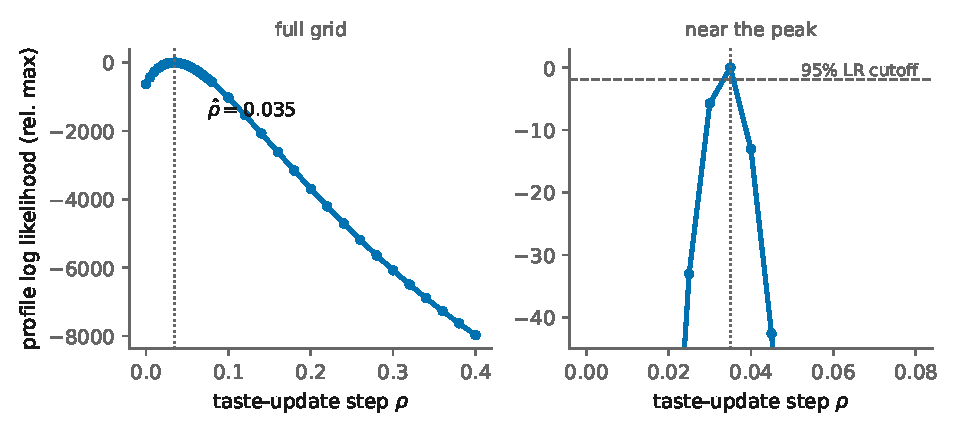
\includegraphics{fig_profile_rho.pdf}
\caption{Profile log likelihood over $\rho$. The dashed line is the 95\%
likelihood-ratio cutoff.}
\label{fig:profile}
\end{figure}

Figure~\ref{fig:profile} shows the result: $\hat\rho=\rhohat$ with 95\% profile
CI [\rhocilo, \rhocihi] (local quadratic approximation; the likelihood-ratio
interval is narrower than the 0.005 grid step, though user clustering widens it
somewhat), and the likelihood ratio against $\rho=0$ is \LRrho.
The taste-shift effect we documented in reduced form in March survives structural
discipline: tastes move, the movement is statistically unambiguous, and a single
click moves the state by about \rhohat\ of the distance to the clicked category.
At $\hat\rho$ the dev-window alignment coefficient is \kappadev\ (SE \kappadevse),
consistent with the training-window estimate.

Two specification checks probe the transition's two strong assumptions, and an
independent adversarial re-analysis of this estimation (placebo tests, cluster
bootstrap, from-scratch reproduction) sharpened both. First, the model says
taste moves only on consumption. Adding a separate update $\rho_{ns}$ for
shown-not-clicked items, evaluated at $\hat\rho$, yields
$\hat\rho_{ns}=\rhonshat$ with a likelihood ratio of \LRns\ against
$\rho_{ns}=0$: declined recommendations push taste \emph{away} from their
category, the backfire effect from our March report, now visible inside the
structural transition. (Because we subsample shown items one-in-ten, the
per-actual-impression step is roughly ten times smaller; the sign and
significance are unambiguous, the structural magnitude is
sampling-convention-dependent.) Movement-only-on-consumption is a workable
first-order approximation, but the backfire term is real, and it matters below
for the simulation's economics. (One honest wrinkle: on a coarse joint grid
the likelihood is willing to trade the click update against backfire, so the
two updates are partially confounded; the profile at $\hat\rho$ is the cleaner
read.)

Second, the constant-$\rho$ update is tested against a diminishing-weight
alternative in which each click carries weight $1/(n_0+t)$, the running-mean
model in which updating slows as histories grow. The running mean fits better,
by \runmeandelta\ log-likelihood points at $n_0=20$, and the adversarial
re-analysis located the source: the best-fit constant $\rho$ falls with a
user's history length almost exactly as $1/(N+T/2)$, which is what Bayesian
posterior updating of a \emph{stable} taste would produce. Within a 14-day
window, ``tastes move with step $\rho$'' and ``the platform's measurement of a
fixed taste sharpens with each observation'' are observationally close, and
MIND favors the second reading at the margin. For the group this cuts two
ways. For calibration it is benign: over this horizon the two updates
prescribe nearly identical dynamics (with prior mass $n_0=20$ and
\(\sim\)7.6 in-window clicks, the running-mean weights sit within a few
thousandths of $\hat\rho$), so
$\hat\rho=\rhohat$ is the right simulation input either way. For the paper it
is a caveat to state: $\rho$ is not a universal taste-plasticity constant but
an effective update rate that declines with user tenure, and separating true
preference drift from belief updating needs either longer panels or exogenous
exposure variation.

\section{The cost of cultivation blindness}\label{sec:sim}

The July 22 meeting converged on the flagship numerical claim: a policy that
ignores cultivation, treating tastes as static, should perform materially worse
than one that plans through the taste dynamics. The simulation tests this in the
calibrated environment: $n=\simItems$ items (the largest categories, with their
estimated $\hat\alpha_c$), $\kappa=\kappahat$, horizon $H=\simH$, initial states
drawn from the empirical distribution of MIND user histories, and $\rho$ swept
over a grid containing $\hat\rho$. Four policies cross two dimensions, knowledge
and planning. Oracle policies know all parameters; learning policies know
$\kappa$ and $\rho$ but must learn the intercepts $\alpha$ across episodes by
maximum likelihood, the estimate-then-plug-in benchmark from Meichun's note.
Aware policies plan through the transition (depth-2 lookahead with a fluid
rollout continuation; an independent adversarial audit verified this planner
recovers the exact dynamic-programming value on every discriminating test
instance, including instances where dynamic planning beats myopic by 28\%);
blind policies recommend the myopically best item under static tastes. All
policies face common random numbers, so at $\rho=0$ aware and blind coincide by
construction and any gap is measured noise-free.

\subsection{Uniform margins: an honest null}

With MIND's own limitation, no revenue data, the baseline scenario sets $m_i=1$
and measures clicks. Table~\ref{tab:sim} shows the result we did not script:
\emph{cultivation blindness costs essentially nothing at the calibrated
parameters}. At $\hat\rho=\rhohat$ the oracle-aware policy earns \clkoa\ clicks
per user against \clkob\ for oracle-blind, and the difference stays within
Monte Carlo noise over the entire $\rho$ grid, even at $\rho=\rhomax$, ten times
the estimated speed. The aware oracle departs from the myopic action in only
\bridgeshare\% of periods at $\hat\rho$. Myopic recommendation is near-optimal
in this regime, for a transparent reason: with uniform margins, the item that
is best to recommend now (high $\alpha_c$ plus high alignment) is also the item
whose basin the platform is happy to drift into, so there is nothing worth
steering against. Expected clicks do rise with $\rho$ for every policy, from
\clkoa\ at $\hat\rho$ toward higher values at large $\rho$: taste dynamics
create value through passive self-reinforcement (the +243\% amplification we
measured in March), but a myopic policy harvests that value for free.

\begin{table}[ht]
\centering
\caption{Uniform-margin scenario: expected clicks per user (H=\simH, \simEp\
users per cell, 5 seeds). The last column is the oracle aware$-$blind gap in
percent; every gap is economically negligible.}
\label{tab:sim}
\begin{tabular}{rrrrrr}
\toprule
$\rho$ & oracle-aware & oracle-blind & learn-aware & learn-blind & gap \\
\midrule
0.000 & 1.96 & 1.96 & 1.90 & 1.90 & 0.0\% \\
0.035 & 2.01 & 2.01 & 1.96 & 1.96 & 0.0\% \\
0.050 & 2.02 & 2.02 & 1.97 & 1.98 & 0.0\% \\
0.150 & 2.17 & 2.17 & 2.10 & 2.11 & 0.0\% \\
0.250 & 2.36 & 2.36 & 2.30 & 2.31 & 0.1\% \\
0.350 & 2.50 & 2.49 & 2.41 & 2.43 & 0.3\% \\
\bottomrule

\end{tabular}
\end{table}

This null is informative, not disappointing, and it is exactly the theory's own
prediction. In Jiangze's classification, bridge items exist when margins and
taste-popularity are misaligned, when the item worth harvesting is not the item
the user would drift to on their own; Meichun's June examples generate bridges
precisely from margin-feature inconsistency. Uniform margins remove the
misalignment, so the model itself says cultivation should be worthless there.
The MIND calibration turns that comparative static into a quantitative
statement about a real platform's parameter regime.

\subsection{Margin misalignment is not enough}

The natural repair is to restore margin-popularity misalignment with
illustrative per-click margins reflecting display-advertising value differences
across verticals (news 1.0 up to finance 4.0), keeping every estimated
parameter unchanged. Table~\ref{tab:simhet} reports revenue per user. The gap
barely moves: \hgaporpct\% at $\hat\rho$ and only \hgapmaxpct\% even at
$\rho=\rhomax$, ten times the estimated plasticity. Pushing on the two other
obvious levers does not change the verdict. Extending the horizon to $H=120$
recommendations yields \hsweepgap\% at $\rho=0.15$; and a high-engagement
counterfactual that shifts every intercept up by 3 log-odds units (mean
consumption probability near one half, a streaming platform rather than a news
feed, with the taste-displacement budget $\rho\,\kappa\,\E[\text{clicks}]$
now of order one) still produces gaps below \egapmaxpct\%.

\begin{table}[ht]
\centering
\caption{Heterogeneous-margin scenario: expected revenue per user (H=\simH,
\simEp\ users per cell, 5 seeds). The last column is the oracle aware$-$blind
gap in percent.}
\label{tab:simhet}
\begin{tabular}{rrrrrr}
\toprule
$\rho$ & oracle-aware & oracle-blind & learn-aware & learn-blind & gap \\
\midrule
0.000 & 4.46 & 4.46 & 4.07 & 4.07 & 0.0\% \\
0.035 & 4.55 & 4.55 & 4.11 & 4.10 & 0.0\% \\
0.050 & 4.65 & 4.65 & 4.21 & 4.24 & 0.0\% \\
0.150 & 5.10 & 5.09 & 4.55 & 4.65 & 0.1\% \\
0.250 & 5.65 & 5.64 & 5.00 & 5.08 & 0.3\% \\
0.350 & 6.19 & 6.16 & 5.50 & 5.58 & 0.5\% \\
\bottomrule

\end{tabular}
\end{table}

\subsection{The reachability gate: why myopic keeps winning, and where it stops}

The simulations expose a structural property of the model that we had not
articulated: \emph{failures are dynamically free}. A declined recommendation
leaves the taste state unchanged, so a policy that wants the user at the
high-margin category can simply recommend that category repeatedly; each
failure costs only the foregone myopic margin of the period, and each success
both collects the margin and moves the state. Direct targeting is therefore
itself a cultivation strategy, and it is exactly what the myopic policy does
whenever the margin gap makes the target myopically attractive. A bridge item
can only beat direct targeting when the target is effectively
\emph{unreachable} from the user's current taste, that is, when alignment
sensitivity $\kappa$ is large enough that a misaligned target's consumption
probability is negligible while an intermediate item both consumes well and
moves the state toward the target. This is visible in our own planner
validation instance: with $\kappa=4$ the exact DP beats myopic by 9.7\%, and
our depth-2 planner captures nearly all of that gap; at MIND's category-level
$\hat\kappa=\kappahat$, no calibrated scenario gets close.

Table~\ref{tab:kappa} makes the gate quantitative by sweeping $\kappa$ with
heterogeneous margins and all other parameters at their MIND values.
Cultivation-aware planning is worthless at $\hat\kappa=\kappahat$, still only
about 1\% at $\kappa=5$, and becomes economically meaningful only around
$\kappa\approx\kappathresh$, where the gap reaches \kgapmidpct\% at
$\rho=0.15$. The gate is sharp, which is itself useful: it says the model's
cultivation economics turn on one measurable quantity.

\begin{table}[ht]
\centering
\caption{The reachability gate: oracle aware$-$blind revenue gap (\%) as
alignment sensitivity $\kappa$ varies, heterogeneous margins, all other
parameters calibrated. MIND sits in the first row.}
\label{tab:kappa}
\begin{tabular}{rrr}
\toprule
$\kappa$ & gap at $\rho=\rhohat$ & gap at $\rho=0.15$ \\
\midrule
1.75 & 0.0\% & 0.1\% \\
3.00 & 0.0\% & 0.3\% \\
5.00 & 0.1\% & 1.0\% \\
7.00 & 0.3\% & 9.9\% \\
\bottomrule

\end{tabular}
\end{table}

Three remarks keep this result in perspective. First, $\hat\kappa$ is
category-level: 18 coarse types compress within-category taste, and a finer
item-level representation would mechanically carry a larger effective
$\kappa$, since alignment then discriminates much more sharply between items.
Whether real platforms sit above the gate is exactly the kind of question the
group can now pose precisely. Second, the backfire effect we estimate
($\hat\rho_{ns}<0$) breaks the failures-are-free property: with backfire,
failed direct targeting actively damages the state, which is precisely what
makes bridges valuable. A model with the estimated backfire term should
generate strictly more cultivation value than the baseline, and that is a
concrete, data-motivated theory extension. Third, learning costs remain small
throughout (learn-aware tracks oracle-aware because with $n=\simItems$ items
and observable states the intercepts are learned within a few hundred
episodes), so the economics are dominated by the planning question, not the
estimation question.

\section{Takeaways for August 5}\label{sec:take}

\begin{enumerate}
\item \textbf{The model's primitives survive structural estimation.} Alignment
drives clicks ($\hat\kappa=\kappahat$, LR \LRkappa) and tastes move on clicks
($\hat\rho=\rhohat$, LR \LRrho). The movement is slow, which vindicates our
caution about magnitudes, but it is statistically unambiguous and the
constant-step linear transition is an adequate local description of it.
\item \textbf{Two data-driven refinements for the model.} Declined
recommendations push taste away ($\hat\rho_{ns}=\rhonshat$ at $\hat\rho$, LR
\LRns), and the update step shrinks with user tenure following the
$1/(N+T/2)$ signature of Bayesian updating of stable tastes. Both are
interpretable and both matter: backfire makes failures costly, which is
precisely the ingredient that restores bridge-item value in the simulation
(takeaway 3), and the tenure effect says cultivation, if it exists, is
front-loaded in a user's lifetime and observationally entangled with the
platform learning the user.
\item \textbf{The flagship claim fails at calibrated parameters, and the
failure is more interesting than the claim.} Cultivation blindness costs
essentially nothing in every calibrated scenario: uniform margins, 4:1 margin
misalignment, high engagement, $H=120$. The reason is structural: failures
leave the state unchanged, so direct targeting is itself the best cultivator
and myopic planning inherits almost all dynamic value. Cultivation-aware
planning pays only above a reachability gate in alignment sensitivity
(gap $\approx\kgapmidpct$\% at $\kappa\approx\kappathresh$ versus
$\hat\kappa=\kappahat$ at the category level). Two honest routes forward:
argue for a finer taste representation with higher effective $\kappa$, or add
the backfire term the data support, which makes failures costly and bridges
valuable. Either way the paper's simulation section should present the gate,
not a universal blindness tax.
\item \textbf{Caveats to state.} Category-level tastes compress items to 18
types; MIND has no margins, so the heterogeneous-margin and engagement
scenarios are counterfactual calibrations; the 14-day window bounds how much
cultivation the data can express; position effects within impressions are not
modeled; the likelihood-ratio statistics treat impression items as
independent, whereas they cluster within users (a cluster bootstrap keeps
every conclusion but shrinks the effective statistics roughly threefold); and
both $\hat\kappa$ and $\hat\rho$ are measured under MSN's incumbent
recommender, whose own next-day exposure tracks recent clicks at least as
strongly as clicking does, so they are policy-dependent behavioral quantities,
the right inputs for calibrating an incumbent-platform simulation and the
wrong ones to read as invariant taste primitives.
\end{enumerate}

\end{document}
